
\documentclass[11pt,a4paper]{article}

\usepackage[utf8]{inputenc} 
\usepackage[T1]{fontenc} 
\usepackage{lmodern}
\usepackage{tcolorbox}

\usepackage[german]{babel}


\setlength{\parindent}{0pt}
\setlength{\parskip}{1ex plus 0.5ex minus 0.5ex}

\usepackage{amsmath} 


\usepackage{graphicx} 

\usepackage[section]{placeins}
\usepackage{booktabs}


\usepackage{hyperref}
\hypersetup{
	colorlinks,
	citecolor=red,
	filecolor=black,
	linkcolor=black,
	urlcolor=black}
\graphicspath{}


\begin{document}



{
	\centering 
	\large 
	Physiklabor für Anfänger*innen \\
	Ferienpraktikum im Sommersemester 2018 \\[4mm]
	\textbf{\LARGE 
		Versuch 19: Gekoppelte Pendel
	} \\[3mm]
	(durchgeführt am 19.09.2018 bei Adrian Hauber) \\
	Ye Joon Kim, Marouan Zouari\\
	\today \\[10mm]
}
\tableofcontents
\newpage
\section{Einleitung}
Die Bewegung gekoppelter Pendel kann dadurch beschrieben werden, indem man deren Bewegungsgleichungen aufstellt. Es wirken insgesamt zwei Kräfte auf ein Pendel, die Gravitationskraft $F_G = mg\sin(\varphi)$ (Zum Pendel senkrechte Komponente) und die Federkraft $F_D = D(x_1 - x_2)$. Mit $M = I\ddot{\varphi}$ und $\vec{M} = \vec{F}\times \vec{r}$lauten beide Bewegungsgleichungen:
$$ I \ddot{\varphi_1} = -mg\sin(\varphi_1)L - D(x_1-x_2)l$$
$$I \ddot{\varphi_2} = -mg\sin(\varphi_2)L - D(x_2-x_1)l$$
Mit $x_i = l\sin{\varphi_i}$ und der Kleinwinkelnäherung sind die Bewegungsgleichungen:
\begin{equation}
\left\{
\begin{array}{c}
I\ddot{\varphi_1}=-mg\varphi_1L - Dl^2(\varphi_1-\varphi_2)
\\
I\ddot{\varphi_2}=-mg\varphi_2L - Dl^2(\varphi_2-\varphi_1)
\end{array}
\right.
\end{equation}

Diese gekoppelte Differenzialgleichungen lassen sich mit einem Variabelaustausch lösen. Nämlich mit $y_1 = \varphi_1 + \varphi_2$ und $y_2 = \varphi_1 - \varphi_2$. Das liefert:
$$\ddot{y_1} = \frac{mgL}{I}y_1$$
$$\ddot{y_2} = \frac{mgL-2Dl^2}{I}y_2$$

Die Pendel wurden als Mathematische Pendel angenähert. Für eine Punktmasse ist ihr Trägheitsmoment $I = mr^2$, wobei $r$ der Abstand von der Rotationsachse zu der Masse ist (In diesem Fall $L$). Eingesetzt in die obigen Formeln liefert:
\begin{equation}
\left\{
\begin{array}{c}
\ddot{y_1} = \frac{g}{L}y_1
\\
\ddot{y_2} = (\frac{g}{L}-\frac{2Dl^2}{mL^2})y_2
\end{array}
\right.
\end{equation}

Beide stellen Gleichungen von Harmonischen Oszillatoren mit den Kreisfrequenzen:
$$ \omega_1^2 = \frac{g}{L}$$
$$ \omega_2^2 = \frac{g}{L}-\frac{2Dl^2}{mL^2} $$
dar.
Diese zwei Kreisfrequenzen entsprechen gleich- und gegensinnigen Schwingungen. 

\section{Ziel des Versuchs}
Das Ziel des Versuchs ist es, die Schwingungsdauer bei gleich- und gegensinnigen Schwingungen sowie die Schwebungsdauer bei verschiedenen Kopplungsgrade zu bestimmen. 
\section{Aufbau}
Für den Versuch wurden zwei mit einer Feder gebundene Pendel benutzt. Beide Seiten der Feder konnten entlang den Pendel verschoben werden, um den Kopplungsgrad zu ändern. 
(Siehe Abb.1)
\begin{figure}
	\centering
	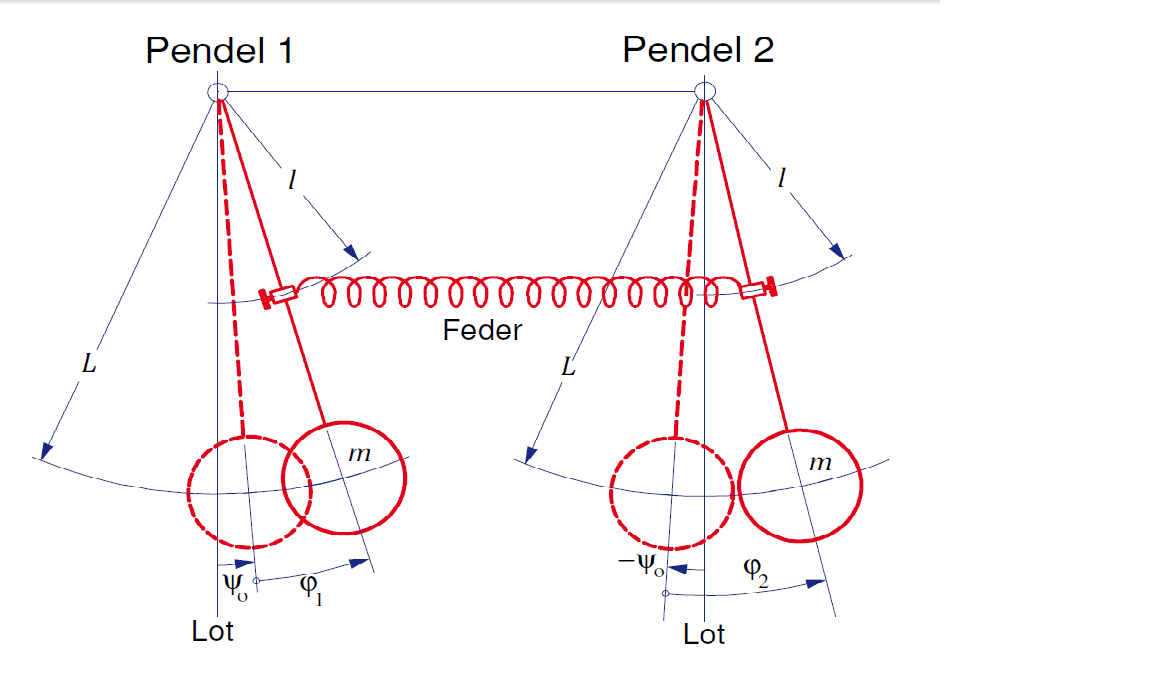
\includegraphics[scale=0.5]{ver19}
	\caption { Gekoppelte Pendel. (,,Versuchsanleitungen'') }
\end{figure}

\section{Durchführung}
Zuerst wurde es sichergestellt, ob die Schwingungsdauer von beiden Pendel die gleiche waren. Die Pendel wurden entkoppelt und die Dauer für vier Schwingungen für beide Pendel wurde mit der Stoppuhr gemessen. Die Positionen der Gewichte an den Pendeln wurden nicht geändert, da es gab zwischen beiden Zeitmessungen fast keinen Unterschied (0,06 Sekunde Abweichung).

Danach wurden die beiden Pendel durch die Feder gekoppelt, und in eine Richtung um 4 cm von ihren Ruhelagen mit zwei von den drei verstellbaren Füße verschoben, um die Schwingungsdauer bei gleichsinniger Schwingung zu messen. Die Pendel wurden gleichzeitig losgelassen, indem man die Füße dreht. Die Zeitmessung wurde angefangen, als einer der Pendel schon eine Schwingung gemacht und ihren Umkehrpunkt erreicht hatte. Es wurde die Zeit für 20 Schwingungen gemessen. 

Die Pendel wurden dann um 4cm in andere Richtungen verschoben. Die Zeitmessungen wurden erneut wie oben durchgeführt. 

Für die Messung der Schwebungsdauer wurde nur eine der Pendel um 4cm nach innen verschoben. Die Zeitmessung wurde angefangen, sobald die verschobene Pendel losgelassen wurde. Die Zeit wurde bis dem zweiten Stillstand der anderen Pendel (die ursprünglich an der Ruhelage war) gemessen. Der Prozesse wurde fünfmal wiederholt. 

Die Lage der Feder an den Pendel wurde dann verschoben, um einen unterschiedlichen Kopplungsgrad einzustellen. Es wurde sichergestellt, dass beide Ende der Feder gleich hoch waren. Die Schwingungsdauer und Schwebungsdauer wurden wie in den letzten zwei Abschnitte erklärt gemessen. Das wurde für vier verschiedene Kopplungsgrade wiederholt. 

\section{Auswertung und Fehleranalyse}
Die Mittelwerte der Schwingungsdauer bei gleichsinnigen Schwingungen, $T_A$, bei gegensinnigen Schwingungen $T_B$, und der Schwebungsdauer $T_S$ für alle Kopplungsgrade und deren Unsicherheiten sind in Tabelle 1 zu sehen. 
\begin{table} [h]
	\begin{tabular*}{0.99\textwidth}{@{\extracolsep{\fill}}c|cccccc}
		\toprule
		$l$ & $T_A$ & $u_{T_A}$ & $T_B$ & $u_{T_B}$ & $T_S$ & $u_{T_S}$  \\
		m & s & s & s & s & s & s   \\
		\bottomrule
		0,705 & 1,63 & 0,02 & 1,874 & 0,009 & 25,4 & 0,3 \\
		0,556 & 1,674 & 0,003 & 1,86 & 0,01 & 33,3 & 0,3 \\
		0,455 & 1,74 & 0,03 & 1,858 & 0,008 & 56,1 & 0,3\\
		0,855 & 1,538 & 0,002 & 1,86 & 0,001 & 18,0 & 0,2 \\
		\bottomrule
	\end{tabular*}
	\caption{Werte für $T_A$, $T_B$ und $T_S$ bei verschiedenen Kopplungsgrade und deren Unsicherheiten.}
\end{table}
\subsubsection{Berechnung}
Um die mittleren Werte für $T_A$ und $T_B$ zu bestimmen wurden die drei Gesamt-Schwingungsdauern summiert und dann durch 60, die totale Anzahl Schwingungen, geteilt. Für deren Unsicherheiten wurde die folgende Formel benutzt:
$$ s_{\bar{x}} = \frac{s_x}{\sqrt{n}}$$
Wobei $s_x$ die Streuung der Mittelwerte ist. Die Streuung der Mittelwerte wurde mit der Formel für Standardunsicherheiten bestimmt, nämlich:
$$s_x=\sqrt{\frac{\sum_{i=1}^{n}(x_i-\bar{x})^2}{n-1}}$$

Die Unsicherheiten der Längen betragen 0,001 m. 

\subsection{Berechnung der theoretischen Schwebungsdauer}
Mit den Werten für $T_A$ und $T_B$ kann der theoretische Wert für $T_S$ berechnet werden, nämlich:
$$\omega_S = \frac{1}{2}(\omega_A-\omega_B)$$
Mit der Substitution $\omega = \frac{2\pi}{T}$ und einer Umformung lässt sich $T_S$ in Terme von $T_A$ und $T_B$ schreiben:
\begin{equation}
T_S = 2\frac{T_A T_B}{T_B-T_A}
\end{equation}
Die berechneten $T_S$ sind:

\begin{table}[h]
	\centering
	\begin{tabular*}{0.99\textwidth}{@{\extracolsep{\fill}}cccc}
		\toprule
		$l$ & $T_S$ & $u_{T_S}$  \\
		m & s & s   \\
		\bottomrule
		0,705 & 24,6 & 2,5 \\
		0,556 & 33,4 & 1,7 \\
		0,455 & 56 & 14,9 \\
		0,855 & 17,86 & 0,14 \\
		\bottomrule
	\end{tabular*}
	\caption{Die mit der Formel berechnete Schwebungsdauer für verschiedene Kopplungsgrade}
	\label{tabelle}
\end{table}

Die Unsicherheiten der Werte lassen sich mit der gauß'schen Fehlerfortpflanzung berechnen. Mit:
$$f(T_A,T_B) = 2\frac{T_A T_B}{T_B-T_A}$$ 
sind
$$\frac{\partial f}{\partial T_A} = 2\frac{T_B^2}{(T_A-T_B)^2}$$
$$\frac{\partial f}{\partial T_B} = -2\frac{T_A^2}{(T_B-T_A)^2}$$

Die Unsicherheiten von $T_S$ sind deshalb:
$$u_{T_S} = \sqrt{(\frac{\partial f}{\partial T_A}u_{T_A})^2+(\frac{\partial f}{\partial T_B}u_{T_B})^2}$$

\subsection{Bestimmung der Kopplungsgrade}
Der Kopplungsgrad lässt sich mit der folgenden Formel berechnen:
\begin{equation}
K = \frac{T_B^2-T_A^2}{T_B^2+T_A^2}
\end{equation}

Die berechnete Werte dafür für jede Messreihe und deren Unsicherheiten sind: 
\begin{table}[h]
	\centering
	\begin{tabular*}{0.99\textwidth}{@{\extracolsep{\fill}}cccc}
		\toprule
		$l$ & $K$ & $u_{K}$  \\
		m &  &    \\
		\bottomrule
		0,705 & 0,14 & 0,01 \\
		0,556 & 0,105 & 0,005 \\
		0,455 & 0,06 & 0,01 \\
		0,855 & 0,187 & 0,007 \\
		\bottomrule
	\end{tabular*}
	\caption{Die mit der Formel berechnete Schwebungsdauer für verschiedene Kopplungsgrade}
	\label{tabelle}
\end{table}

Die Unsicherheiten lassen sich wiederum mit der gauß'schen Fehlerfortpflanzung berechnen. Mit:
$$f(T_A,T_B) = \frac{T_B^2-T_A^2}{T_B^2+T_A^2}$$
sind
$$\frac{\partial f}{\partial T_A} = -\frac{4T_A T_B^2}{(T_A^2+T_B^2)^2}$$
$$\frac{\partial f}{\partial T_B} = \frac{4T_A^2 T_B}{(T_B^2+T_A^2)^2}$$
Die Unsicherheiten von $K$ sind deshalb:
$$u_{K} = \sqrt{(\frac{\partial f}{\partial T_A}u_{T_A})^2+(\frac{\partial f}{\partial T_B}u_{T_B})^2}$$

Eine lineare Regression wurde dann mit einem Excel-Dokument gemacht, um zu sehen, ob es eine lineare Zusammenhang zwischen $l^2$ und $K$ gibt. Die lineare Gleichung lautet:
$$ K = a\cdot l^2 +b = 0,2327 l^2 + 0,02 $$
Mit den Unsicherheiten: $u_a = 0,01$ und $u_b = 0,03$ (Siehe Abbildung 1). 
\begin{figure}[h]
	\centering
	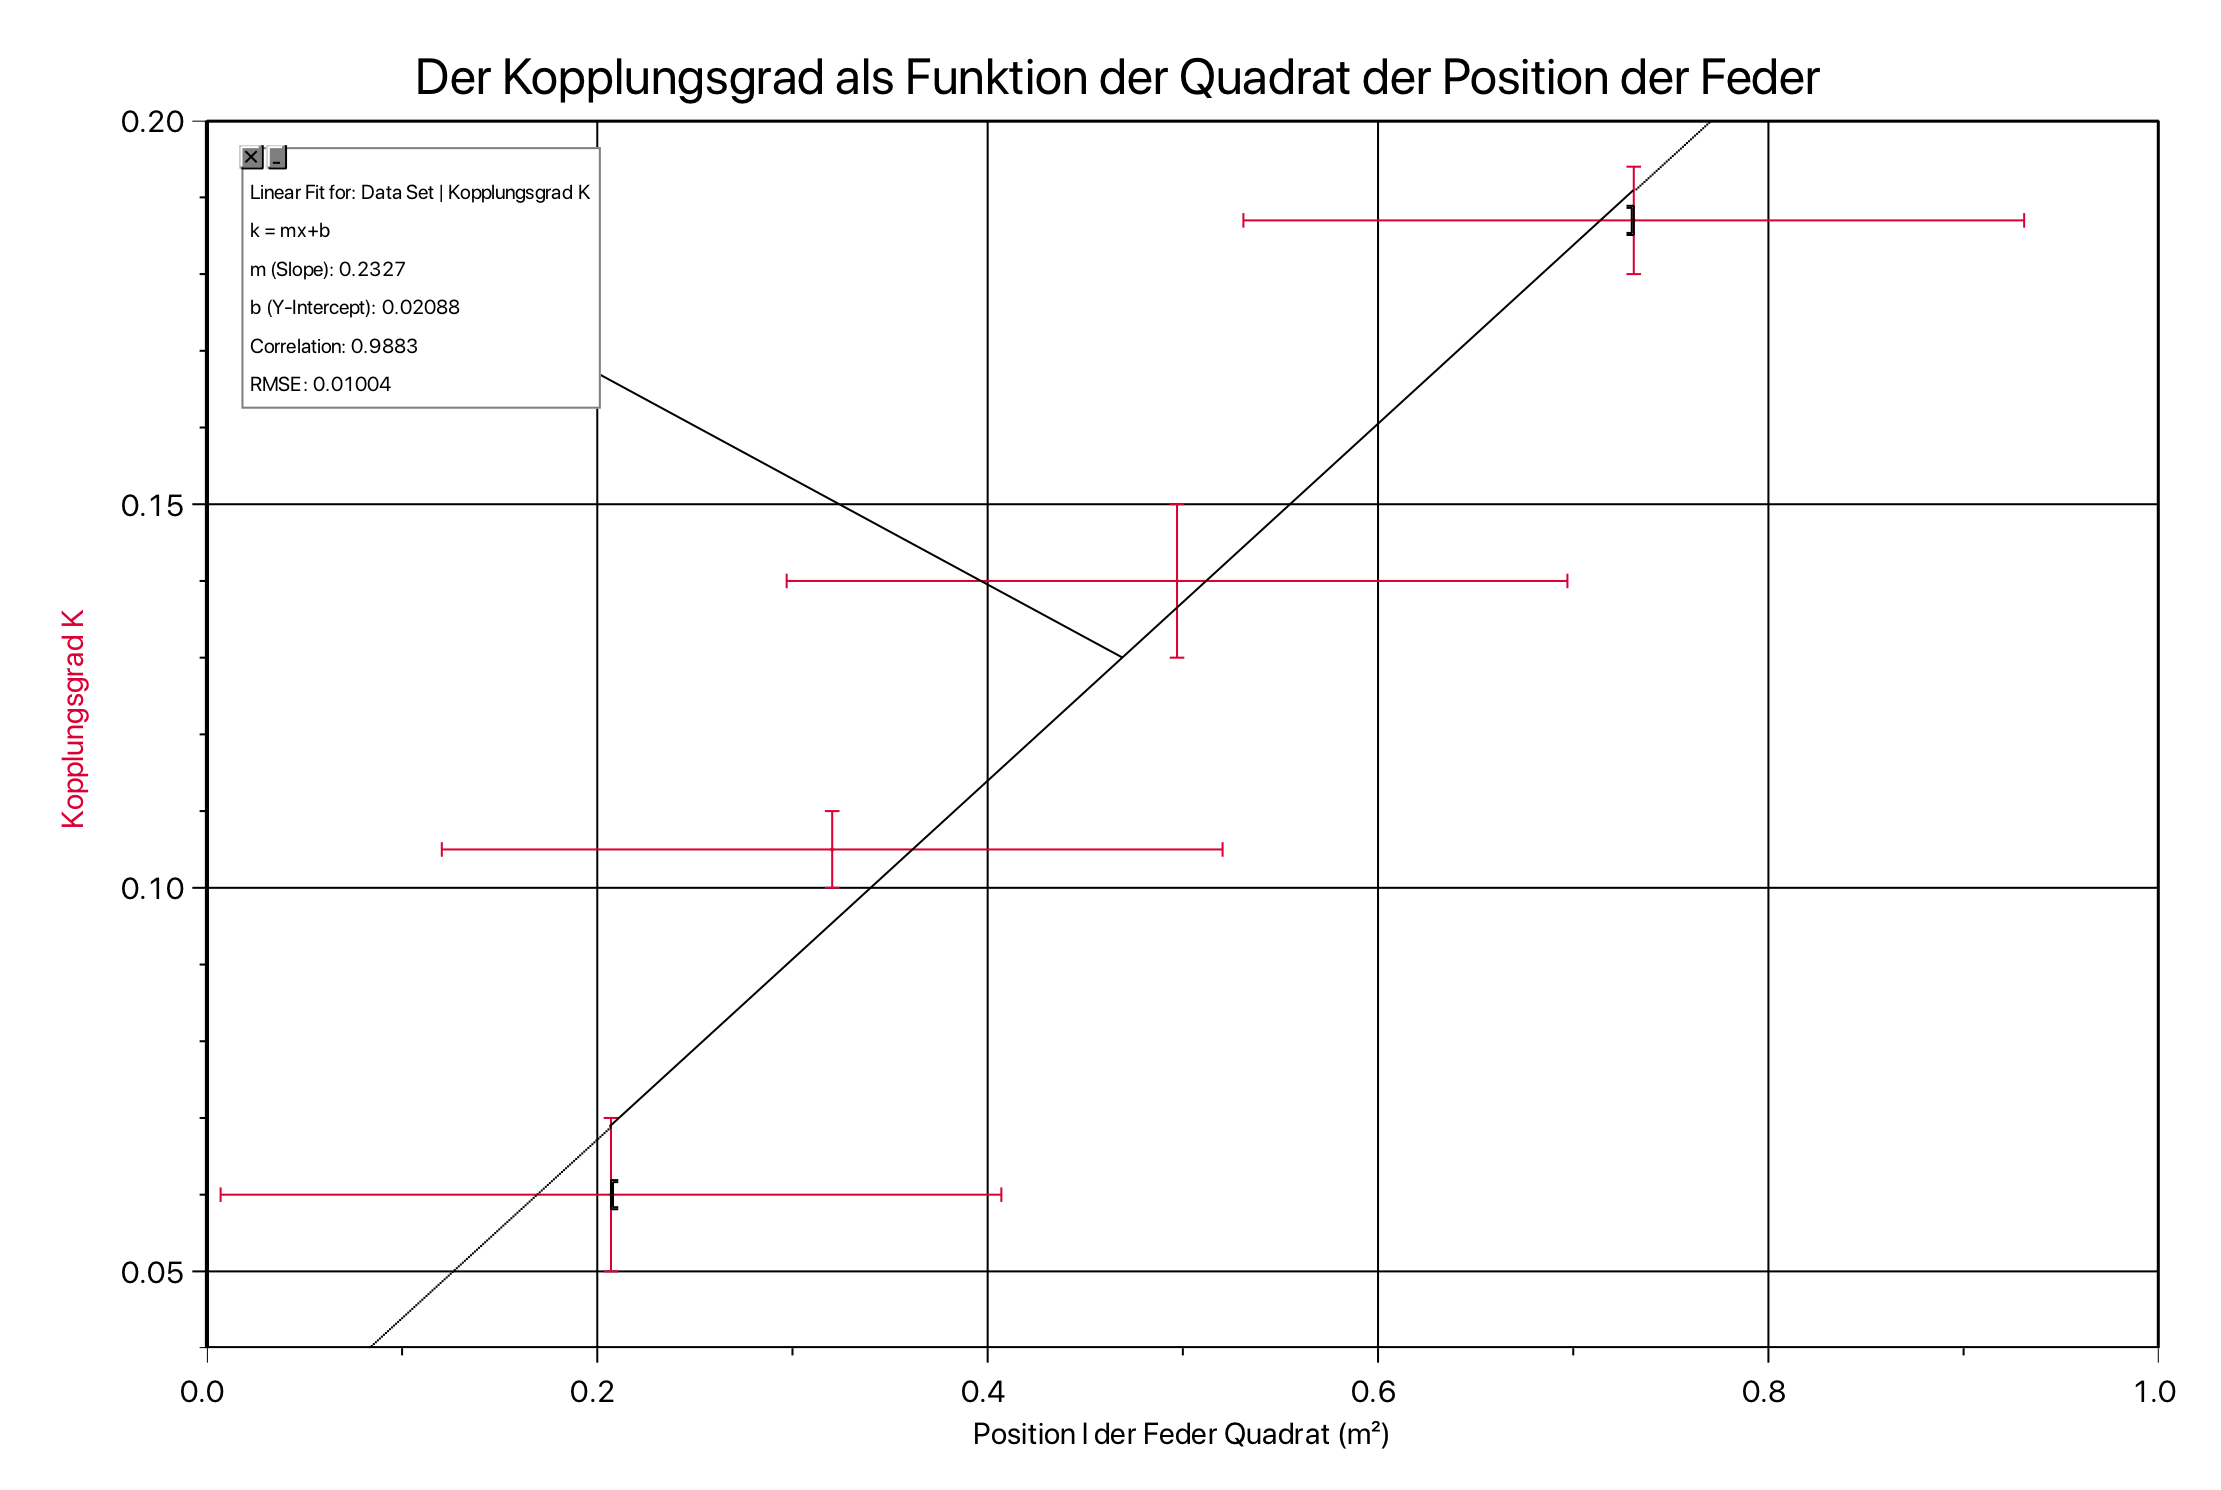
\includegraphics[width=\textwidth]{Abb2}
	\caption{Eine Graph von $K$ als Funktion von $l^2$}
\end{figure}

\section{Diskussion der Ergebnisse}
\subsection{Systematische und statistische Fehler}
Ein systematischer Fehler entsteht dadurch, dass die Feder eine nicht ideale Feder ist.
Dann w"urde es Abweichungen von der linearen Beziehung zwischen Kraft und Abstand geben. Daher wird die verwendete Gleichung eine schlechte Annäherung sein bzw. ein schlechtes Modell für diesen Fall darstellen.
\\\
Außerdem würde das gleiche Problem entstehen, wenn die Feder zwischen den beiden Pendel nicht perfekt horizontal ist, oder wenn die anfangs gew"ahlte Amplitude sehr groß ist.

Für dieses Experiment können verschiedene statistische Fehlerquellen vorliegen.
\\\
Zum Beispiel, die Anzahl der Oszillationen mit bloßem Auge zu messen, und die Tatsache, dass die Zeitmessung vom menschlichen Reflex sehr abh"angig ist sind auch wichtige Fehlerquellen. 
\subsection{Diskussion "uber die gefundene Werten}
Die Werte von $T_S$ f"ur verschiedene $l$, die durch das Experiment bestimmt wurden, stimmen mit den berechneten Theoretische Werten "uberein, weil sie innerhalb ihrer Unsicherheiten liegen.
\\\
Aber die Unsicherheiten der Theoretischen Werten, außer f"ur $l=0.855 m$ und $l=0,556$, sind hoch, da sie sind ungefähr 10 Prozent der entsprechenden Werte. Deshalb sind diese Werte nicht von großer Bedeutung.
\\\
Es wurde bestimmt, dass es eine lineare Zusammenhang zwischen $k$ und $l^2$ gibt, mit :
$$ K = a\cdot l^2 +b = 0,2327 l^2 + 0,02 $$

Die Korrelation, die von dem Programm Logger Pro berechnet wurde, war 0,9883, was sehr nah an 1 liegt. Deswegen gibt es einen klaren linearen Zusammenhang, jedoch sind die Werte für die Steigung und Achsenabschnitt relativ unsicher, da die horizontalen Fehlerbalken der einzelnen Punkte wegen der Fehlerfortpflanzung sehr groß geworden sind. Es können deshalb mehrere lineare Regressionen gezeichnet werden, die alle durch die Fehlerbalken gehen. Insgesamt kann es sichergestellt werden, dass es einen linearen Zusammenhang zwischen $k$ und $l^2$ gibt, aber die Steigungen und Achsenabschitte der jeweiligen Gleichungen sind nicht genau bestimmt.
\subsection{Verbesserungsvorschläge}
Die Statistischen Fehler k"onnten dadurch reduziert werden, dass man ein System benutzt, das automatisch die Anzahl der Schwingungen bzw. der Schwebungen zählt und deren Dauer misst. 
\\\
Der Schutz der Feder vor äußerem Einfluss (wie z.B extreme Temperaturen und Kr"afte...) und angemessene Wahl der Amplitude sind Methoden, um systematische Fehler zu vermeiden und verringern.
\section{Literatur und Bildquellen}
,,Versuchsanleitungen zum Physiklabor für Anfänger*innen, Teil 1.''  Albert-Ludwigs-Universität Freiburg: 2018. 


\section{Anhang}
Siehe Zusatzblatt




\end{document}